% PACKAGES ARE NOT SUPPORTED
%\section{Packages description}
%\label{sec:Packages}

%\subsection{Packages structure}
%Despite the fact that we recommend users to install the complete COMPSs Framework, we have built different packages to allow users
%customize as maximum as possible their installation. Figure \ref{fig:compss_packages_debian} illustrates the COMPSs 
%packaging structure and its internal dependencies. 
%\begin{figure}[ht!]
%  \centering
%    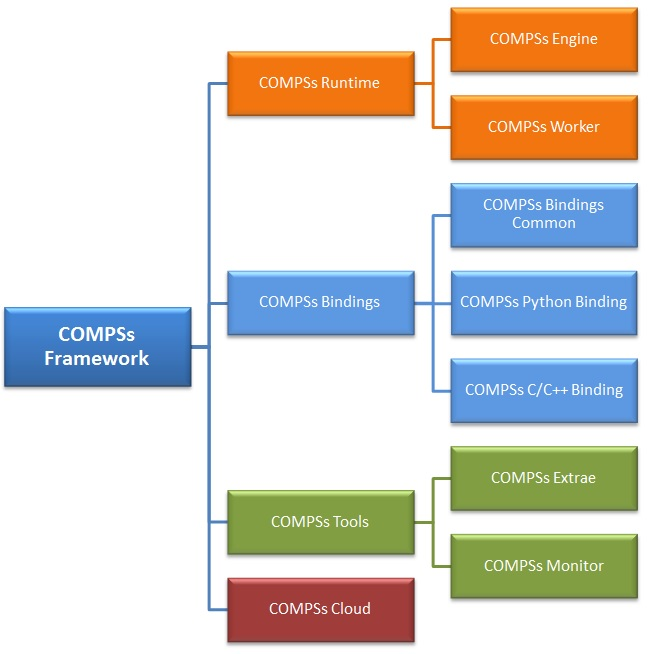
\includegraphics[width=0.75\textwidth]{./Sections/02_Packages_Description/Figures/compss_packages.jpeg}
%    \caption{COMPSs packaging structure}
%    \label{fig:compss_packages_debian}
%\end{figure}
%
%\newpage

\section{Dependencies}
\label{subsec:packages_dependencies}
Next we provide a list of dependencies for installing COMPSs package. The exact names may vary depending on 
the Linux distribution but this list provides a general overview of the COMPSs dependencies. For specific information about
your distribution please check the \textit{Depends} section at your package manager (apt, yum, zypper, etc.).

\bgroup
  \def\arraystretch{1.5}
  \begin{center}
    \begin{tabular}{ p{6cm} | p{10cm} } 
    COMPSs Runtime 		& openjdk-8-jre, graphviz, xdg-utils, openssh-server \\ \hline  
    COMPSs Python Binding 	& libtool, automake, build-essential, python ($>= 2.7$ | $>=3.6$), python-dev | python3-dev, python-setuptools| python3-setuptools, libpython2.7 \\ \hline 
    COMPSs C/C++ Binding 	& libtool, automake, build-essential, libboost-all-dev, libxml2-dev \\ \hline
    COMPSs Autoparallel		& libgmp3-dev, flex, bison, libbison-dev, texinfo, libffi-dev, astor, sympy, enum34, islpy \\ \hline
    COMPSs Tracing 		& libxml2 ($>= 2.5$), libxml2-dev ($>= 2.5$), gfortran, papi \\ \hline   
    \end{tabular}
  \end{center}
\egroup

\subsection{Build Dependencies}

To build COMPSs from sources you will also need \verb|wget|, \verb|openjdk-8-jdk| and \verb|maven|.

\subsection{Optional Dependencies}

For the Python binding it is also recommended to have \verb|dill| and \verb|guppy| installed. The \verb|dill| package increases
the variety of serializable objects by Python (for example: lambda functions), and the \verb|guppy| package is needed to use the \verb|@local|
decorator. Both packages can be found in pyPI and can be installed via \verb|pip|.
